\section{Our Systems}

In this section, we describe two systems we implemented -- a conventional entity-centric classifier and an end-to-end neural network. While \newcite{hermann2015teaching} do provide several baselines for performance on the RC task, we suspect that their baselines are not that strong. They attempt to use a frame-semantic parser, and we feel that the poor coverage of that parser undermines the results, and is not representative of what a straightforward NLP system -- based on standard approaches to factoid question answering and relation extraction developed over the last 15 years -- can achieve. Indeed, their frame-semantic model is markedly inferior to another baseline they provide, a heuristic word distance model. At present just two papers are available presenting results on this RC task, both presenting neural network approaches: \cite{hermann2015teaching} and \cite{hill2016goldilocks}. While the latter is wrapped in the language of end-to-end memory networks, it actually presents a fairly simple window-based neural network classifier running on the CNN data. Its success again raises questions about the true nature and complexity of the RC task provided by this dataset, which we seek to clarify by building a simple attention-based neural net classifier.

Given the (passage, question, answer) triple $(p, q, a)$, $p = \{p_1, \ldots, p_{m}\}$ and $q = \{q_1, \ldots, q_{l}\}$ are sequences of tokens for the passage and question sentence, with $q$ containing exactly one ``@placeholder'' token. The goal is to infer the correct entity $a \in p \cap E$ that the placeholder corresponds to, where $E$ is the set of all abstract entity markers. Note that the correct answer entity must appear in the passage $p$.

\subsection{Entity-Centric Classifier}

We first build a conventional feature-based classifier, aiming to explore what features are effective for this task. This is similar in spirit to \cite{wang2015machine}, which at present has very competitive performance on the MCTest RC dataset \cite{richardson2013mctest}. The setup of this system is to design a feature vector $f_{p, q}(e)$ for each candidate entity $e$, and to learn a weight vector $\theta$ such that the correct answer $a$ is expected to rank higher than all other candidate entities:
\begin{equation}
\theta^{\intercal}f_{p, q}(a) > \theta^{\intercal}f_{p, q}(e), \forall e \in E \cap p \setminus \{a\}
\end{equation}

We employ the following feature templates:
\begin{enumerate}[1.]
    \setlength\itemsep{-0.1em}
    \item
        Whether entity $e$ occurs in the passage.
    \item
        Whether entity $e$ occurs in the question.
    \item
        The frequency of entity $e$ in the passage.
    \item
        The first position of occurence of entity $e$ in the passage.
    \item
        $n$-gram exact match: whether there is an exact match between the text surrounding the placeholder and the text surrounding entity $e$. We have features for all combinations of matching left and/or right one or two words.
    \item
        Word distance: we align the placeholder with each occurrence of entity $e$, and compute the average minimum distance of each non-stop question word from the entity in the passage.
    \item
        Sentence co-occurrence: whether entity $e$ co-occurs with another entity or verb that appears in the question, in some sentence of the passage.
    \item
        Dependency parse match: we dependency parse both the question and all the sentences in the passage, and extract an indicator feature of whether $w \xrightarrow{r} \text{@placeholder}$ and $w \xrightarrow{r} e$ are both found; similar features are constructed for $\text{@placeholder} \xrightarrow{r} w$ and $e \xrightarrow{r} w$.
\end{enumerate}



\subsection{End-to-end Neural Network}

Our neural network system is based on the \ti{AttentiveReader} model proposed by \cite{hermann2015teaching}. The framework can be described in the following three steps (see Figure \ref{fig:framework}):

\begin{figure*}[!ht]
\centering
    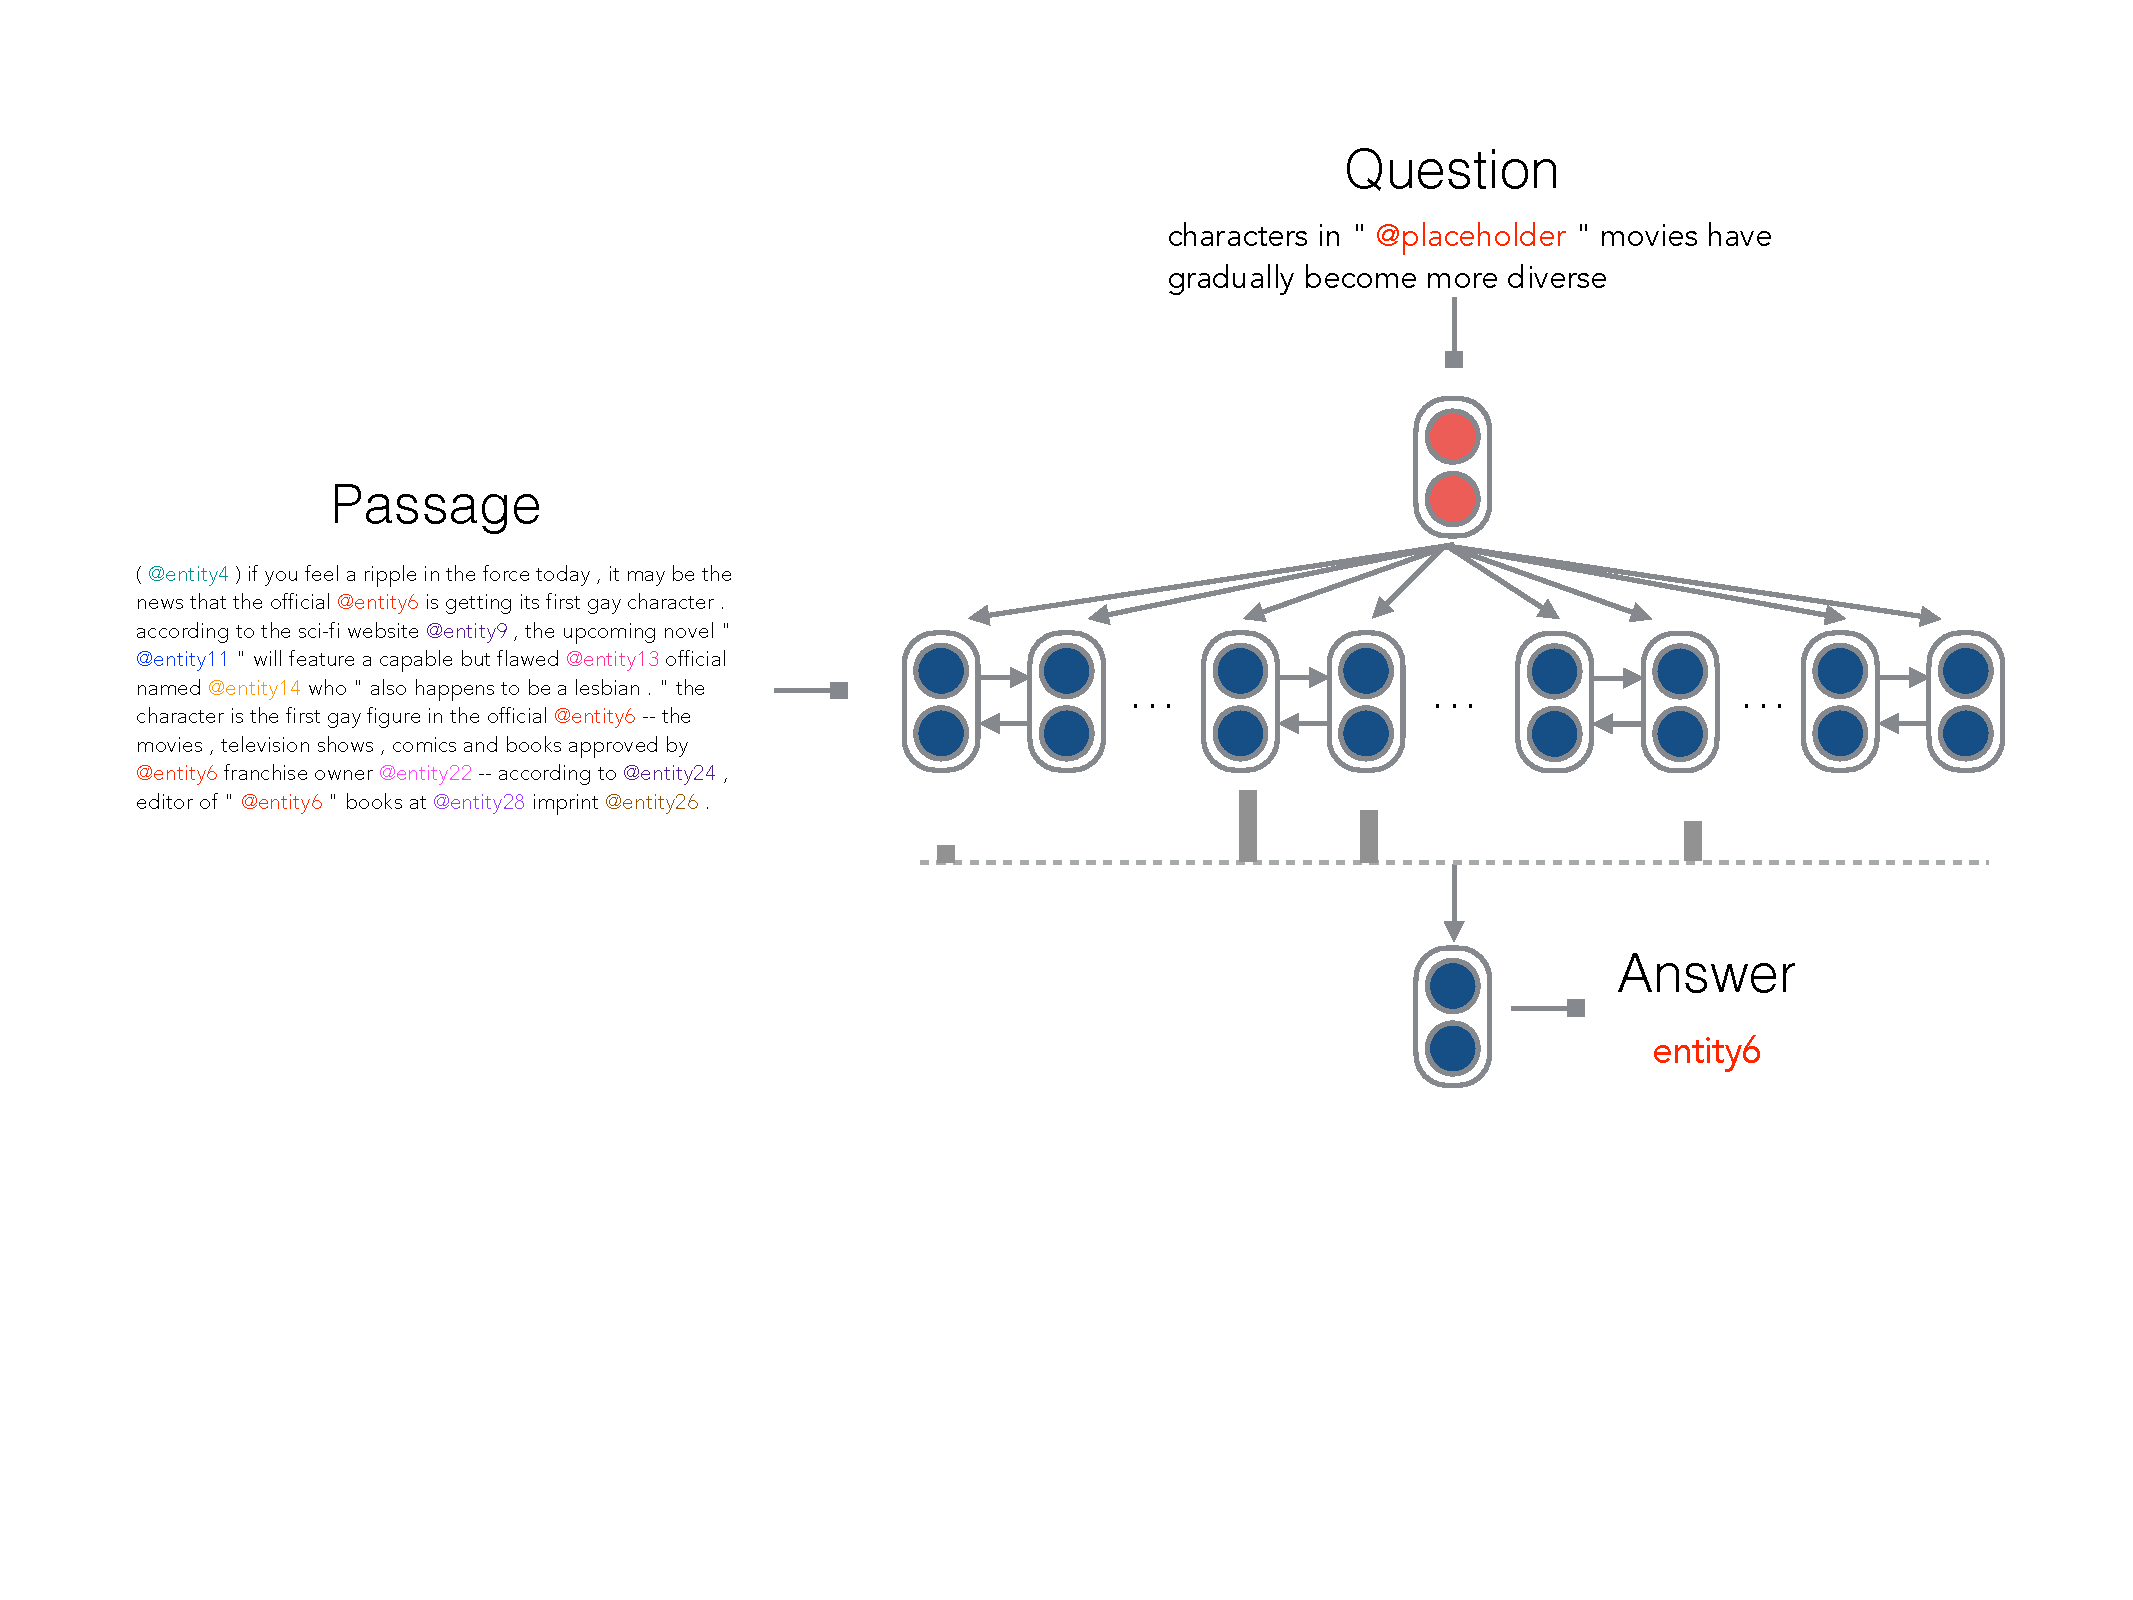
\includegraphics[scale=0.37]{figures/fig_model.pdf}
\caption{Our neural network architecture for the reading comprehension task.}
\label{fig:framework}
\end{figure*}

\begin{description}
    \item[\tf{Encoding:}] First, all the words are mapped to $d$-dimensional vectors via an embedding matrix $E \in \R^{d \times |\mathcal{V}|}$; therefore we have $p$: $\mf{p}_1, \ldots, \mf{p}_m \in R^d$ and $q: \mf{q}_1, \ldots, \mf{q}_{l} \in R^d$.

        Next we use a shallow bi-directional recurrent neural network (RNN) with hidden size $\tilde{h}$ to encode contextual embeddings $\tilde{\mf{p}}_i$ of each word in the passage,
        \begin{eqnarray*}
            \overrightarrow{\mf{h}}_i & = & \text{RNN}(\overrightarrow{\mf{h}}_{i-1}, \mf{p}_i), i = 1, \ldots, m\\
            \overleftarrow{\mf{h}}_i & = & \text{RNN}(\overleftarrow{\mf{h}}_{i+1}, \mf{p}_i), i = m, \ldots, 1
        \end{eqnarray*}
        and $\tilde{\mf{p}}_i = \text{concat}(\overrightarrow{\mf{h}}_i, \overleftarrow{\mf{h}}_i) \in \R^{h}$, where $h = 2 \tilde{h}$.
        Meanwhile, we use another bi-directional RNN to map the question $\mf{q}_1, \ldots, \mf{q}_l$ to an embedding $\mf{q} \in \R^h$. We choose to use Gated Recurrent Unit (GRU) \cite{cho2014learning} in our experiments because it performs similarly but is computationally cheaper than LSTM.

    \item[\tf{Attention:}] In this step, the goal is to compare the question embedding and all the contextual embeddings, and \ti{select} the pieces of information that are relevant to the question. We compute a probability distribution $\alpha$ depending on the degree of relevance between word $p_i$ (in its context) and the question $q$ and then produce an output vector $\mf{o}$ which is a weighted combination of all contextual embeddings $\{\tilde{\mf{p}}_i\}$:
        \begin{eqnarray}
            \alpha_i & = & \softmax\nolimits_i \mf{q} ^{\intercal} \mf{W}_{s} \tilde{\mf{p}}_i  \\
            \mf{o} & = & \sum\nolimits_{i}{\alpha_i \tilde{\mf{p}}_i}
        \end{eqnarray}
        $\mf{W_s} \in \R^{h \times h}$ is used in a bilinear term, which allows us to compute a similarity between $\mf{q}$ and $\tilde{\mf{p}}_i$ more flexibly than with just a dot product.
    \item[\tf{Prediction:}] Using the \ti{output} vector $\mf{o}$, the system outputs the most likely answer using:
        \begin{equation}
            a = \argmax\nolimits_{a \in p \cap E}{W_a ^{\intercal} \mf{o}}
        \end{equation}
        Finally, the system adds a softmax function on top of $W_a ^{\intercal} \mf{o}$ and adopts a negative log-likelihood objective for training.
\end{description}

\paragraph*{Differences from \cite{hermann2015teaching}.}
Our model basically follows the \ti{AttentiveReader}. However, to our surprise, our experiments observed nearly \tf{7} --\tf{10}\% improvement over the original \ti{AttentiveReader} results on \ti{CNN} and \ti{Daily Mail} datasets (discussed in Sec.~\ref{sec:experiments}). Concretely, our model has the following differences:
\begin{itemize}
\item
We use a bilinear term, instead of a $\tanh$ layer to compute the relevance (attention) between question and contextual embeddings. The effectiveness of the simple bilinear attention function has been shown previously for neural machine translation by \cite{luong2015effective}.
\item
After obtaining the weighted contextual embeddings $\mf{o}$, we use $\mf{o}$ for direct prediction. In contrast, the original model in \cite{hermann2015teaching} combined $\mf{o}$ and the question embedding $\mf{q}$ via another non-linear layer before making final predictions. We found that we could remove this layer without harming performance. We believe it is sufficient for the model to learn to return the entity to which it maximally gives attention.
\item
The original model considers all the words from the vocabulary $\mathcal{V}$ in making predictions. We think this is unnecessary, and only predict among entities which appear in the passage.
\end{itemize}
Of these changes, only the first seems important; the other two just aim at keeping the model simple.

\paragraph*{Window-based MemN2Ns \cite{hill2016goldilocks}.}
Another recent neural network approach proposed by \cite{hill2016goldilocks} is based on a memory network architecture \cite{weston2015memory}. We think it is highly similar in spirit. The biggest difference is their way of encoding passages: they demonstrate that it is most effective to only use a 5-word context window when evaluating a candidate entity and they use a positional unigram approach to encode the contextual embeddings: if a window consists of 5 words $x_1, \ldots, x_5$, then it is encoded as $\sum_{i=1}^{5}{E_i(x_i)}$, resulting in $5$ separate embedding matrices to learn. They encode the 5-word window surrounding the placeholder in a similar way and all other words in the question text are ignored. In addition, they simply use a dot product to compute the ``relevance'' between the question and a contextual embedding. This simple model nevertheless works well, showing the extent to which this RC task can be done by very local context matching.
